% !TeX program = lualatex
\documentclass[DIV=12, parskip=half, fontsize=12pt, a4paper]{scrartcl}

%\usepackage[utf8]{inputenc}
%\usepackage[T1]{fontenc}    % Font-Encoding
\usepackage{lmodern}        % LModern font
\usepackage[ngerman]{babel} % deutsche Lokalisierung
%\usepackage{graphicx}       % Einbindung von Bildern
\usepackage{pdfpages}


\usepackage{lineno}         % Nummerierung der Zeilen
%\usepackage{csquotes}       % bessere Anführungszeichen
%\usepackage{eurosym}        % Euro-Zeichen setzen
%\usepackage[normalem]{ulem} % Durchstreichen von Text-Passagen
%\usepackage[shortlabels]{enumitem} % bessere Aufzählungen mit Kurzschreibweise der Labels

\usepackage{pdfpages}       % erlaubt das Einbinden von Seiten anderer PDF-Dateien


\usepackage{draftwatermark}
\SetWatermarkText{Entwurf}


\title{Änderungsantrag zum Antrag zur Änderung der Wahlordnung für die Wahlen der Fachschaftsvertretungen und Fachschaftsräte (FSWO)}
\author{Fachschaftenkonferenz}
\date{\today}

\begin{document}

	\maketitle
	Das SP möge auf Vorschlag der Fachschaftenkonferenz beschließen:

	\begin{linenumbers}
		Der Antrag zur Änderung der Wahlordnung für die Wahlen der Fachschaftsvertretungen und Fachschaftsräte (FSWO) vom 7. Oktober 2019 (im 41. SP als Antrag 48/41 in 1. Lesung in der 11. ordentlichen Sitzung am 20.11.2019 diskutiert und im 42. SP erneut in 1. Lesung in der 1. ordentlichen Sitzung am 26.02.2020 diskutiert) wird wie folgt neugefasst:

		\begin{center}\bfseries\LARGE Antrag zur Neufassung der Fachschaftswahlordnung
		\end{center}

		Das SP möge auf Vorschlag der Fachschaftenkonferenz beschließen:

		Die Wahlordnung für die Wahlen der Fachschaftsvertretungen und Fachschaftsräte der Studierendenschaft der Rheinischen Friedrich-Wilhelms-Universität Bonn vom 16. Mai 2017 wird durch die beigefügte Wahlordnung geändert und neugefasst.

		Die neugefasste Wahlordnung tritt mit ihrer Veröffentlichung auf der Bekanntmachungsplattform der Studierendenschaft in Kraft.

		Mit Inkrafttreten der neugefassten Wahlordnung tritt die Wahlordnung für die Wahlen der Fachschaftsvertretungen und Fachschaftsräte in der Fassung vom 16. Mai 2017 außer Kraft.
		Auf Wahlen, deren Wahlausschuss bereits vor Inkrafttreten dieser Ordnung bestellt wurde, findet die Wahlordnung für die Wahlen der Fachschaftsvertretungen und Fachschaftsräte der Rheinischen Friedrich-Wilhelms-Universität 	Bonn in der Fassung vom 16. Mai 2017 Anwendung.

		Das  SP-Präsidium und das Fachschaftenkolletiv  werden  damit  beauftragt,  diesen Beschluss unverzüglich auszufertigen und zur Veröffentlichung durch die Öffentlichkeitsbeauftragte zu bringen.
	\end{linenumbers}

	\vspace{1em}
	\textit{Ausgefertigt aufgrund des Beschlusses der Fachschaftenkonferenz am dd. November 2020.}

	Bonn, den \today \\
	Christoph Liedel \\
	{\scriptsize Vorsitzender des Fachschaftenkollektivs, Fachschaftenreferent}

	\clearpage
	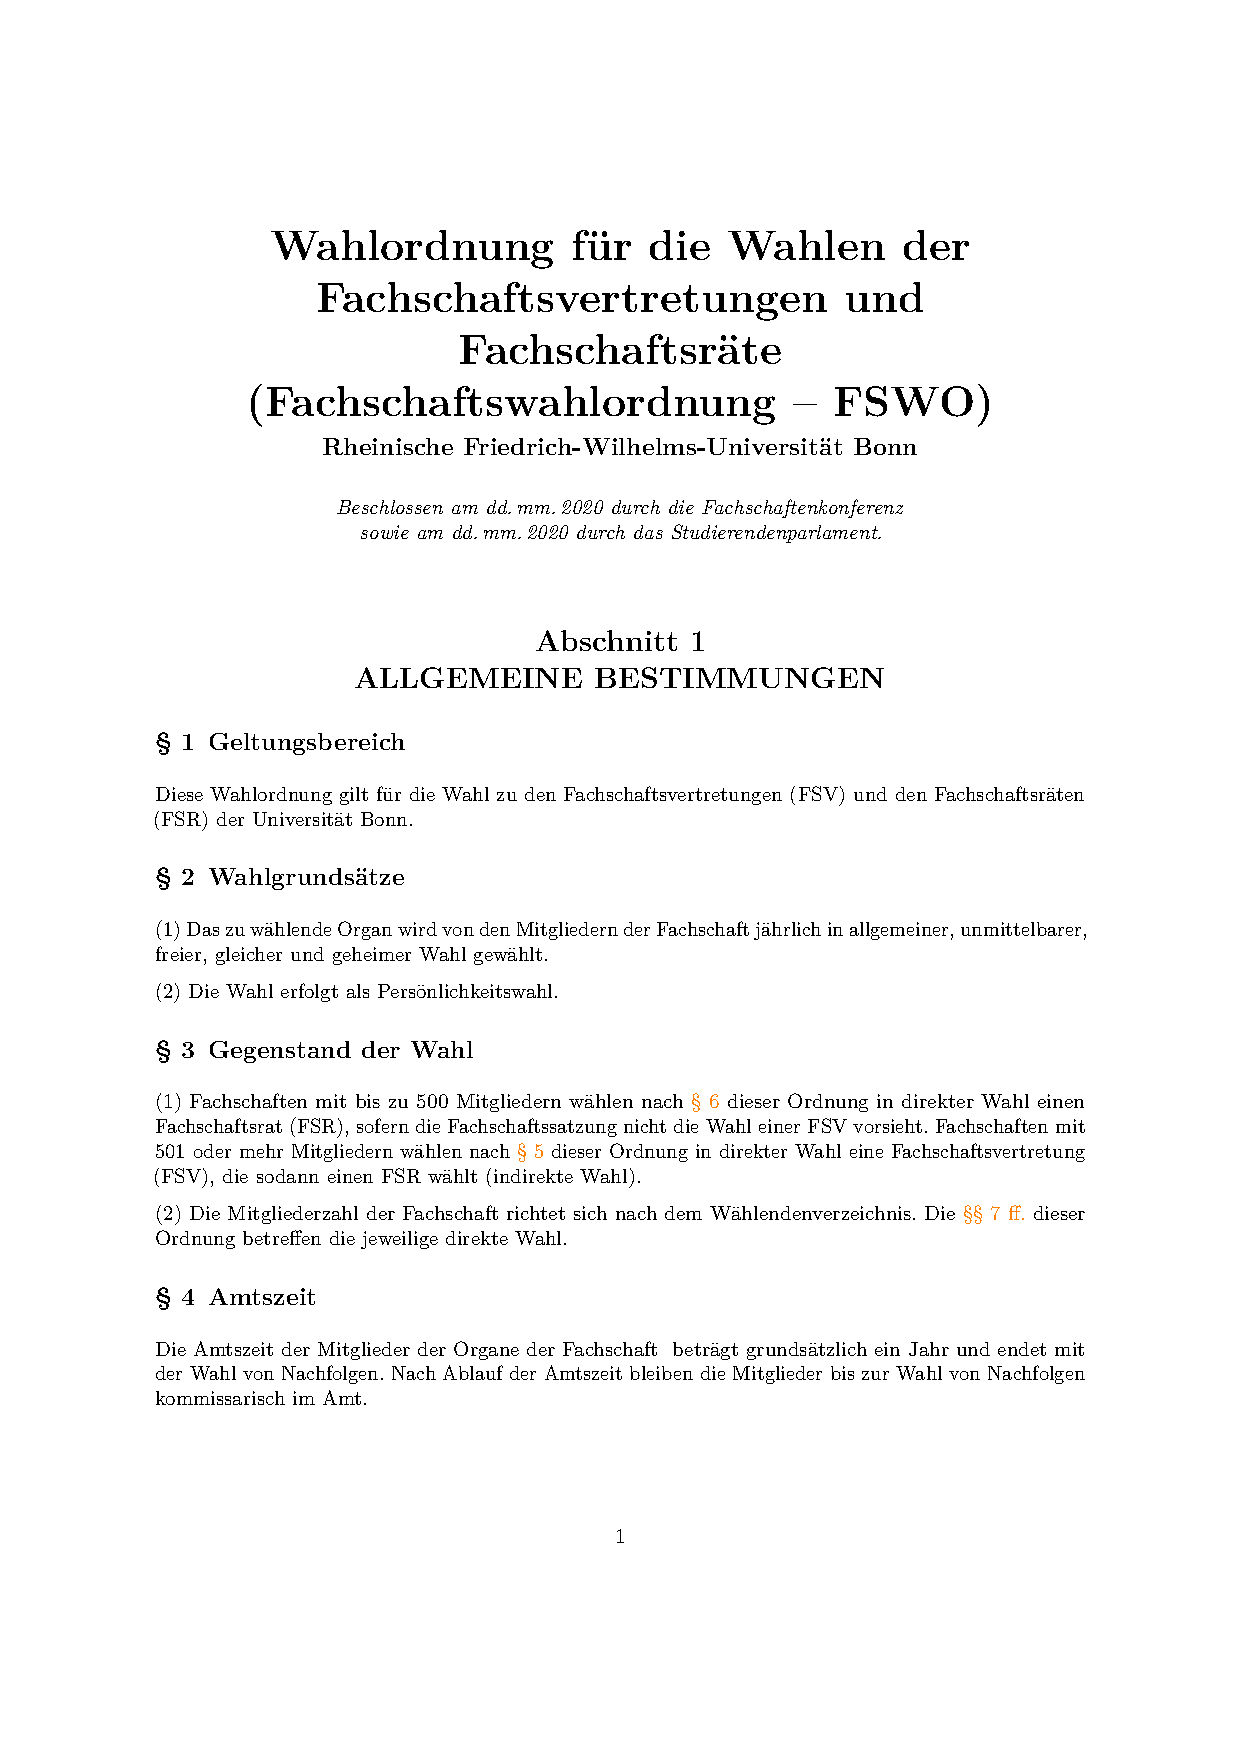
\includepdf[pages=-]{FSWO-Entwurf-ohne-Anmerkungen}
\end{document}
